\section{Barrier functions}

In essence, barrier methods also use the notion of using proxies for the constraints in the objective function, so that an unconstrained optimisation problem can be solved instead. However, the concept of barrier functions is different than penalty functions in that they are defined to \emph{prevent} the solution search method from leaving the feasible region, which is why some of these methods are also called \emph{interior point methods.} 

Consider the primal problem $P$ being defined as
\begin{flalign*}
	(P) :~ \mini \ & f(x) \\ 
	\st & g(x) \leq 0 \\
	&x \in X.
\end{flalign*}

We define the \emph{barrier problem} $BP$ as 
\vspace{-3pt}
	\begin{flalign*}
	(BP) :~ \inf_{\mu} \ & \theta(\mu) \\ 
	\st & \mu > 0 
\end{flalign*}

where $\theta(\mu) = \inf_x\braces{f(x) + \mu B(x) : g(x) < 0, x \in X}$ and $B(x)$ is a \emph{barrier function}. The barrier function is such that its value approaches $+\infty$ as the boundary of the region $\braces{x : g(x) \leq 0}$ is approached from its interior. Notice that, in practice, it means that the constraint $g(x) < 0$ can be dropped, as they are automatically enforced by the barrier function.  

The barrier function $B: \reals^m \rightarrow \reals$ is such that
%
\begin{equation}
B(x) = \sum_{i=1}^m \phi(g_i(x)) \text{, where }
\begin{cases}  
	\phi(y) \geq 0, &\text{ if } y < 0; \\ 
    \phi(y) = +\infty, &\text{ when } y \rightarrow 0^{-}.
\end{cases} \label{eq:barrier_prop}                 
\end{equation}
%
Examples of barrier functions that impose this behaviour are 
\begin{itemize}
\item $B(x) = -\sum_{i=1}^m \frac{1}{g_i(x)}$
\item $B(x) = -\sum_{i=1}^m \ln(\min\braces{1, -g_i(x)})$
\end{itemize}

Perhaps the most important barrier function is the \emph{Frisch's log barrier function}, used in the highly successful primal-dual interior point methods. We will describe its use later. The log barrier is defined as
$$
B(x) = - \sum_{i=1}^m \ln(-g_i(x)). 
$$

Figure \ref{fig:different_mu} illustrates the behaviour of the barrier function. Ideally, the barrier function $B(x)$ has the role of an \emph{indicator function}, which is zero for all feasible solutions $x \in \braces{x : g(x) < 0}$ but assume infinite value if a solution is at the boundary $g(x)=0$ or outside the feasible region. This is illustrated in the dashed line in Figure \ref{fig:different_mu}. The barrier functions for different values of barrier term $\mu$ illustrate how the log barrier mimics this behaviour, becoming more and more pronounced as $\mu$ decreases.

\begin{figure}
	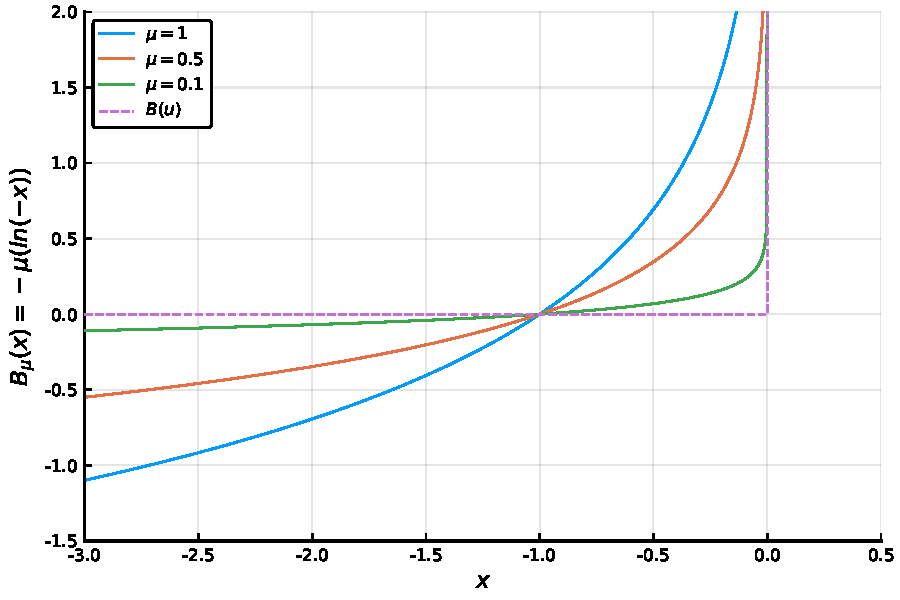
\includegraphics[width=\textwidth]{part_2/chapter_10/figures/different_mu.pdf}
	\caption{The barrier function for different values of $\mu$} \label{fig:different_mu}
\end{figure}

\section{The barrier method}

In a similar nature to what was developed for penalty methods, we can devise a solution method that successively solves the barrier problem $\theta(\mu)$ for decreasing values of the barrier term $\mu$. 

We start by stating the result that guarantees convergence of the barrier method. 

\begin{theorem}[Convergence of barrier methods]\label{thm:convergence}
Let $f:\reals^n\rightarrow \reals$ and $g: \reals^n \rightarrow \reals$ be continuous functions and $X\in\reals^n$ a nonempty closed set in problem $P$. Suppose $\braces{x \in \reals^n : g(x) < 0, x \in X}$ is not empty. Let $\overline{x}$ be the optimal solution of $P$ such that, for any neighbourhood $N_\epsilon(\overline{x}) = \braces {x : ||x - \overline{x}|| \leq \epsilon}$, there exists $x \in X \cap N_\epsilon$ for which $g(x) < 0$. Then
$$
\min\braces{f(x) : g(x) \leq 0, x \in X} = \lim_{\mu \rightarrow 0^+} \theta(\mu) = \inf_{\mu > 0} \theta(\mu).
$$
Letting $\theta(\mu) = f(x_{\mu}) + \mu B(x_{\mu})$, where $B(x)$ is a barrier function as described in \eqref{eq:barrier_prop}, $x_{\mu} \in X$ and $g(x_{\mu}) < 0$, the limit of $\braces{x_{\mu}}$ is optimal to $P$ and $\mu B(x_{\mu})\rightarrow 0$ as $\mu \rightarrow 0^+$.
\end{theorem}

\begin{proof}
First, we show that $\theta(\mu)$ is a nondecreasing function in $\mu$. For $\mu > \lambda > 0$ and $x$ such that $g(x) < 0$ and $x \in X$, we have
%
\begin{align*}
& f(x) + \mu B(x) \geq f(x) + \lambda B(x) \\
& \inf_x \braces{f(x) + \mu B(x)} \geq \inf_x \braces{f(x) + \lambda B(x)} \\
& \theta(\mu)	\geq  \theta(\lambda).
\end{align*}
%
From these, we conclude that $\lim_{\mu \rightarrow 0^+}\theta(\mu)=\inf\braces{\theta(\mu) : \mu > 0}$. Now, let $\epsilon >0$. As $\overline{x}$ is optimal, by assumption there exists some $\hat{x} \in X$ with $g(\hat{x}) < 0$ such that $f(\overline{x}) + \epsilon > f(\hat{x})$. Then, for $\mu > 0$ we have 
%
$$
f(\overline{x}) + \epsilon + \mu B(\hat{x}) > f(\hat{x}) + \mu B(\hat{x}) \geq \theta(\mu).
$$ 
Letting $\mu \rightarrow 0^+$, it follows that $f(\overline{x}) + \epsilon \geq \lim_{\mu \rightarrow 0^+}
\theta(\mu)$, which implies $f(\overline{x}) \geq \lim_{\mu \rightarrow 0^+}\theta(\mu)= \inf\braces{\theta(\mu) : \mu > 0} $. Conversely, since $B(x) \geq 0$ and $g(x) < 0$ for some $\mu > 0$, we have
\begin{align*}
\theta(\mu) &= \inf\braces{f(x) + \mu B(x) : g(x) < 0, x \in X}\\ 
&\geq \inf\braces{f(x) : g(x) < 0, x \in X}\\
&\geq \inf\braces{f(x) : g(x) \leq 0, x \in X} = f(\overline{x}).
\end{align*}
Thus $f(\overline{x}) \leq \lim_{\mu \rightarrow 0^+}\theta(\mu)= \inf\braces{\theta(\mu) : \mu > 0}$. Therefore, $f(\overline{x}) = \lim_{\mu \rightarrow 0^+}\theta(\mu)= \inf\braces{\theta(\mu) : \mu > 0}$.
\end{proof}

The proof has three main steps. First, we show that $\theta(\mu)$ is a nondecreasing function in $\mu$, which implies that $\lim_{\mu \rightarrow 0^+}\theta(\mu)= \inf\braces{\theta(\mu) : \mu > 0}$. This can be trivially shown as only feasible solutions $x$ are required to be considered. 

Next, we show the convergence of the barrier method by showing that $\inf_{\mu > 0}\theta(\mu) = f(\overline{x})$, where $\overline{x} = \arg\min\braces{f(x) : g(x) \leq 0, x \in X} = \lim_{\mu \rightarrow 0^+} \theta(\mu) = \inf_{\mu > 0} \theta(\mu)$. The optimality of $\overline{x}$ implies that $ f(\hat{x}) - f(\overline{x}) < \epsilon$ for feasible $\hat{x}$ and $\epsilon > 0$. Moreover, $B(\hat{x}) \geq 0$ by definition. In the last part, we use the argument that including the boundary can only improve the objective function value, leading to the last inequality. It is worth highlighting that, to simplify the proof, we have assumed that the barrier function has the form described in \eqref{eq:barrier_prop}. However, a proof in the veins of Theorem \ref{thm:convergence} can be still be developed for the Frisch log barrier (for which $B(x)$ is not necessarily nonnegative) since, essentially, \eqref{eq:barrier_prop} only needs to be observed in a neighbourhood of $g(x) = 0$.

The result in Theorem \ref{thm:convergence} allows to design a optimisation methods that, starting from a strictly feasible (interior) solution, is based on successively reducing the barrier term until a solution with arbitrarily small barrier term is obtained. Algorithm \ref{Alg1} present a pseudo code for such method.

\begin{algorithm}[H]
\caption{Barrier method} \label{Alg1}
\begin{algorithmic}[1] %line numbering frequency. 
\State {\bf initialise.} $\epsilon > 0, x^0 \in X \text{ with } g(x^k) < 0, \mu^k, \beta \in (0,1), k = 0$. 
\While {$\mu^kB(x^k) > \epsilon$} 
    \State $\overline{x}^{k+1} = \arg\min \braces{f(x) + \mu^kB(x) : x \in X}$ \label{x-step}
    \State $\mu^{k+1} = \beta\mu^k$, $k = k+1$ 
\EndWhile
\State {\bf return} $x^k$.
\end{algorithmic}
\end{algorithm}

One important aspect to notice is that starting the algorithm requires a strictly feasible point, which in some applications, might be challenging to be obtained. This characteristic is what renders the name \emph{interior point methods} for this class of algorithms. 

Consider the following example. Let $P = \braces{(x+1)^2 : x \ge 0}$. Let us assume that we use the barrier function $B(x) = -\ln(x)$. Then, we unconstrained barrier problem becomes

\begin{equation}
 (BP): \mini_x (x+1)^2 - \mu \ln(x).	
\end{equation}

Since this is a convex function, the first order condition $f'(x) = 0$ is necessary and sufficient for optimality. Thus, solving $2(x+1) - \frac{\mu}{x} = 0$ we obtain the positive root and unique solution $x_\mu=\frac{-1}{2} + \frac{\sqrt{4 + 8\mu}}{4}$. Figure X shows the behaviour of the problem as $\mu$ converges to zero. As can be seen, as $\mu \rightarrow 0$, the optimal solution $x_\mu$ converges to the constrained optimum $\overline{x} = 0$.

\begin{figure}
	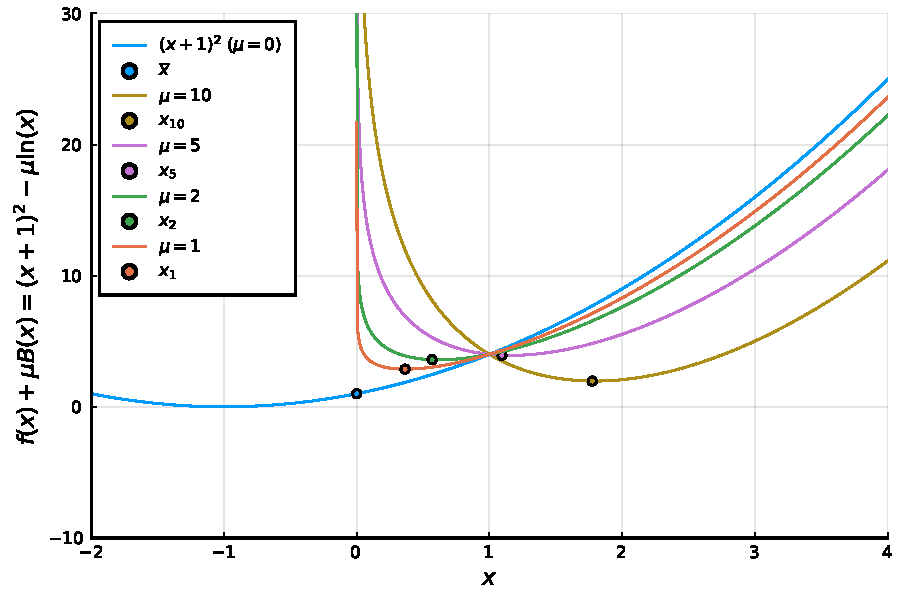
\includegraphics[width=0.8\textwidth]{part_2/chapter_10/figures/ex2-barrier.pdf}
	\caption{Example 1: solving a one-dimensional problem with the barrier method} \label{fig:figure_2}
\end{figure}  

We now consider a more involved example. Let us consider the problem 
$$
	P = \mini\braces{(x_1-2)^4 + (x_1-2x_2)^2 : x_1^2 - x_2 \leq 0}
$$ 
with $B(x) = -\frac{1}{x_1^2 - x_2}$. We implemented Algorithm \ref{Alg1} and solved it with two distinct values for the penalty term $\mu$ and reduction term $\beta$. Figure \ref{fig:figure_2} illustrate the trajectory of the algorithm with each parametrisation, exemplifying how these can affect the convergence of the method.

\begin{figure}[h]
	\center
	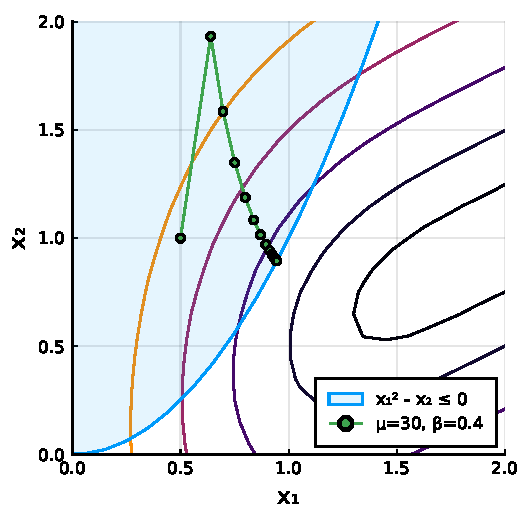
\includegraphics[width = 0.45\textwidth]{part_2/chapter_10/figures/ex3-barrier-1.pdf}
	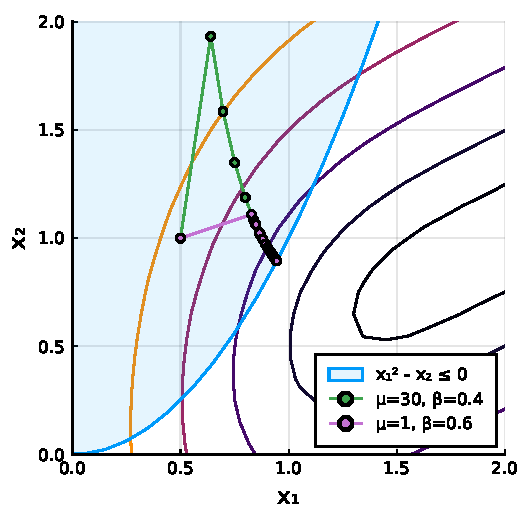
\includegraphics[width = 0.45\textwidth]{part_2/chapter_10/figures/ex3-barrier-2.pdf}
	\caption{The trajectory of the barrier method for problem $P$. Notice how the parameters influence the trajectory and number of iterations. The parameters on the left require 27 iterations while those on the right require 40 iterations for convergence.} \label{fig:barrier_2}
\end{figure}



\section{Interior point method for LP/QP problems}


Perhaps ironically, the most successful applications of barrier methods in terms of efficient implementations are devoted to solving linear and quadratic programming (LP/QP) problems. The primal-dual interior point method has become in the last decade the algorithm of choice for many applications involving large-scale LP/QP problems. 

To see how barrier methods can be applied to LP problems, consider the following primal/dual pair formed by a LP primal $P$
\begin{align*}
(P) ~:~ \mini \ &c^\top x \\
\st &Ax = b \ :v \\
&x \geq 0 \ :u
\end{align*}
%
and its respective dual formulation $D$
%
\begin{align*}
(D) ~:~ \maxi \ &b^\top v \\
\st &A^\top v + u = c \\
&u \geq 0, v \in \reals^m. 
\end{align*}
%
The optimal solution $(\overline{x}, \overline{v}, \overline{u}) = \overline{w}$ is such that it satisfies KKT conditions of $P$, given by
%
\begin{flalign*}
&Ax = b, \ x \geq 0\\ 
&A^\top v + u = c, \ u \geq 0, \ v \in \reals^m\\
&u^\top x = 0. 
\end{flalign*}
%
These are going to be useful as a reference for the next developments. We start by considering the \emph{barrier problem} for $P$ by using the logarithmic barrier function to represent the condition $x \geq 0$. Thus, the barrier problem $BP$ can be defined as
%
\begin{flalign*}
(BP) ~:~ \mini \ &c^\top x  - \mu\sum_{i=1}^n \ln(x_j)\\
\st &Ax = b. 
\end{flalign*}
%
Notice that this problem is a strictly-convex equality constrained problem that is suitable to be solved using the constrained variant of Newton's method (which simply consists of employing Newton's method to solve the KKT conditions of equality constrained problems). Moreover, observe that the KKT conditions of $BP$ are
% 
\begin{flalign*}
&Ax = b, \ x > 0\\ 
&A^\top v = c - \mu\left(\frac{1}{x_1},\dots,\frac{1}{x_n}\right)
\end{flalign*}
%
Notice that, since $\mu > 0$ and $x > 0$, $u = \mu\left(\frac{1}{x_1},\dots,\frac{1}{x_n}\right)$ serves as an estimate for the Lagrangian dual variables. To further understand the relationship between the optimality conditions of $BP$ and $P$, let us define $X\in \reals^{n\times n}$ and $U \in \reals^{n \times n}$ as
$$
X = \diag(x) = \begin{bmatrix} \ddots & & \\   
                                        & x_i & \\
                                        & & \ddots     
                 \end{bmatrix}
                 \text{ and }
  U = \diag(u) = \begin{bmatrix} \ddots & & \\   
                                        & u_i & \\
                                        & & \ddots     
                 \end{bmatrix}               
$$
and let $e = [1,\dots,1]^\top$ be a vector of ones of suitable dimension. We can rewrite the KKT conditions of BP as
%
\begin{flalign}
&Ax = b, \ x > 0 \label{eq:pKKT1}\\ 
&A^\top v + u = c  \label{eq:pKKT2}\\ 
&u = \mu X^{-1}e ~\Rightarrow~ XUe = \mu e. \label{eq:pKKT3}
\end{flalign}
%
Notice how the condition \eqref{eq:pKKT3} resembles the complementary slackness from $P$, but \emph{relaxed} to be $\mu$ instead of zero. This is why this system is often referred to as the \emph{perturbed KKT system}. 

Theorem \ref{thm:convergence}\footnote{In fact, we require a slight variant fo Theorem 1 that allow for $B(x) \geq 0$ only being required in a neighbourhood of $g(x)=0$.} guarantees that $w_\mu = (x_\mu, v_\mu, u_\mu)$ approaches the optimal primal-dual solution of $P$ as $\mu \rightarrow 0^+$. The trajectory formed by successive solutions $\braces{w_\mu}$ is called the \emph{central path}, which is due to the interiority enforced by the barrier function. When the barrier term $\mu$ is large enough, the solution of the barrier problem is close to the analytic centre of the feasibility set. The analytic centre of a polyhedral set $S = \braces{x \in \reals^n : Ax \leq b} $ is given by
%
\begin{align*}
	\maxi_x & \prod_{i=1}^m (b_i - a_i ^\top x) \\
	\st & x \in X, 	
\end{align*}
%	
which corresponds to finding the point of maximum distance to each of the hyperplanes forming the polyhedral set. This is equivalent to the convex problem 
%
\begin{align*}
	\mini_x & \sum_{i=1}^m -\ln(b_i - a_i ^\top x) \\
	\st & x \in X, 	
\end{align*}
%
and thus justifying the nomenclature.

One aspects should be observed for defining stopping criterion. Notice that the term $u^\top x$ is such that it measures the duality gap at a given solution. That is, notice that
\begin{align*}
	c^\top x & = (A^\top v + u)^\top x	\\
	& = (A^\top v)^\top x + u^\top x \\
	& = v^\top(Ax) + u^\top x \\
	c^\top x - b^\top v & = u^\top x = \sum_{i=1}^n u_ix_i = \sum_{i=1}^n \left(\frac{\mu}{x_i}\right)x_i = n\mu.
\end{align*}
%
which gives the \emph{total slack violation} that can be used to determine the convergence of the algorithm.

\subsection{Primal/dual path-following interior point method}

The primal/dual path following interior point method (IPM) is the specialised version of the setting described earlier for solving LP/QP problems. 

It consists of building upon employing logarithmic barriers to LP/QP problems and solving the system \eqref{eq:pKKT1} - \eqref{eq:pKKT3} using Newton's method. However, instead of solving the problem to optimality for each $\mu$, only a \emph{single} Newton step is taken before the barrier term $\mu$ is reduced. 

Suppose we start with a $\overline{\mu} > 0$ and a $w^k = (x^k, v^k, u^k)$ sufficiently close to $w_{\overline{\mu}}$. Then, for a sufficiently small $\beta \in (0,1)$, $\beta\overline{\mu}$ will lead to a $w^{k+1}$ sufficiently close to $w_{\beta\overline{\mu}}$. Figure \ref{fig:approx_central} illustrates this effect, showing how a suboptimal solution $x^k$ do not necessarily need to be in the central path (denoted by the dashed line) to guarantee convergence, as long as they are guaranteed to remain within the some neighbourhood $N_\mu(\theta)$ of the central path.

\begin{figure}[h]
	\begin{tikzpicture}
		\node at (0,0) {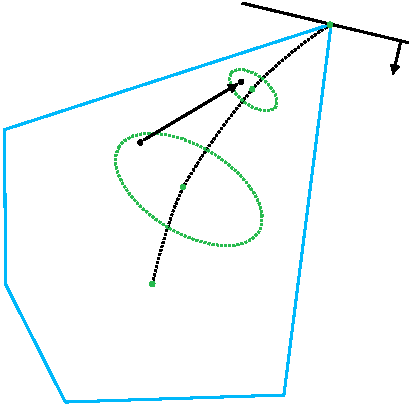
\includegraphics{part_2/chapter_10/figures/central_path_lp.pdf}};
%		\draw[help lines] (-4,-4) grid (4,4);
		\node[below] at (-0.4,-1.2) {$x_{+\infty}$};
		\node[right] at (-0.4,0.2) {$x_{\mu_2}$};		
		\node[below] at (1.15,2.1) {$x_{\mu_1}$};
		\node[right] at (-1.2,0.9) {$x^k$};
		\node[above] at (0.8,2.05) {$x^{k+1}$};
		\node[below] at (3.5,2.6) {$c$};
		\node[below] at (0.4,-0.6) {$N_{\mu_2}(\theta)$};
		\node[below] at (1.1,1.7) {$N_{\mu_1}(\theta)$};	
	\end{tikzpicture}
	\caption{an illustrative representation of the central path and how the IPM follows it approximately. }\label{fig:approx_central}
\end{figure}


For example, let $N_\mu(\theta) = ||X_\mu \, U_\mu e - \mu e|| \leq \theta\mu$. Then, by selecting $\beta = 1 -  \frac{\sigma}{\sqrt{n}}$, $\sigma = \theta = 0.1$, and $\mu^0= (x^\top u)/ n$, successive Newton steps are guaranteed to remain within $N_\mu(\theta)$. 

To see how the setting works, let the perturbed KKT system \eqref{eq:pKKT1} -- \eqref{eq:pKKT3} for each $\hat{\mu}$ be denoted as $H(w) = 0$. Let $J(\overline{w})$ be the Jacobian of $H(w)$ at $\overline{w}$. 

Applying Newton's method to solve $H(w)=0$ for $\overline{w}$, we obtain
\begin{equation}
J(\overline{w})d_w = -H(\overline{w}) \label{eq:NewtonSystem}
\end{equation}
where $d_w = (w - \overline{w})$. By rewriting $d_w = (d_x, d_v, d_u)$, \eqref{eq:NewtonSystem} can be equivalently stated as 
%
\begin{equation}
\begin{bmatrix} A ~\, & 0^{\top} & 0 \\ 0 ~\, & A^\top & I \\ \overline{U} ~\, & 0^{\top} & \overline{X} \end{bmatrix} \begin{bmatrix}d_x \\ d_v \\ d_u \end{bmatrix} =  
\begin{bmatrix}0 \\ 0 \\ \hat{\mu}e - \overline{X} \, \overline{U}e \end{bmatrix}. \label{eq:NewtonSystem_matrix}
\end{equation}
%
The system \eqref{eq:NewtonSystem_matrix} is often referred to as the Newton's system. 

In practice, the updates incorporate primal and dual infeasibility, which precludes the need of additional mechanisms to guarantee primal and dual feasibility throughout the algorithm. This can be achieved with a simple modification in the Newton system, rendering the direction update step
%
\begin{equation}
\begin{bmatrix} A ~\, & 0^{\top} & 0 \\ 
				0 ~\, & A^\top & I \\ 
				U^k ~\, & 0^{\top} & X^k 
\end{bmatrix} 
\begin{bmatrix}d_x^{k+1} \\ 
			   d_v^{k+1} \\ 
			   d_u^{k+1} 
\end{bmatrix} = - 
\begin{bmatrix} Ax^k - b \\ A^\top v^k + u^k - c \\ X^k U^ke -\mu^{k+1}e \end{bmatrix}, \label{eq:update_step}
\end{equation}
 
To see how this still leads to primal and dual feasible solutions, consider the primal residuals (i.e., the amount of infeasibility) as $r_p(x,u,v) = Ax- b$ and the dual residuals $r_d(x,u,v) = A^\top v + u - c$. Now, let $r (w) = r(x,u,v) = (r_p(x,u,v), r_d(x,u,v))$, recalling that  $w^k = (x, v, u)$. The optimality conditions can be expressed as requiring that the residuals must vanish, that is $r(\overline{w}) = 0$.

Now, consider the first-order Taylor approximation for $r$ at $w$ for a step $d_w$
$$
r(w + d_w) \approx r(w) + Dr(w)d_w,
$$
where $Dr(w)$ is the derivative of $r$ evaluated at $w$, which is given by the two first rows of the Newton system \eqref{eq:NewtonSystem_matrix}. The step $d_w$ for which the residue vanishes is
%
\begin{equation}
	Dr(w) d_w = -r(w) \label{eq:Newton_step_residual},	
\end{equation}
%
which is the same as \eqref{eq:NewtonSystem} without the bottom equation. Now, if we consider the directional derivative of the square of the norm of $r$ in the direction $d_w$, we obtain

\begin{equation}
	\left. \frac{d}{dt} || r(w + td_w) ||_2^2 \right|_{t \rightarrow 0^+} = 2r(w)^\top Dr(w)d_w = -2 r(w)^\top r(w),
\end{equation}

which is strictly decreasing. That is, the step $d_w$ is such that it will make the residual decrease and eventually become zero. From that point onwards, the Newton system will take the form of \eqref{eq:NewtonSystem_matrix}.

 
The algorithm proceeds by iteratively solving the system \eqref{eq:update_step} with $\mu^{k+1} = \beta\mu^{k}$ with $\beta \in (0,1)$ until $n\mu^{k}$ is less than a specified tolerance. Algorithm \ref{Alg2} summarises a simplified form of the IPM.
%
\begin{algorithm}[H]
\caption{Interior point method (IPM) for LP} \label{Alg2}
\begin{algorithmic}[1] %line numbering frequency. 
\State {\bf initialise.}\text{ primal-dual feasible} $w^k$, $\epsilon > 0$, $\mu^k$, $\beta \in (0,1)$, $k = 0$. 
\While {$n\mu= c^\top x^k - b^\top v^k > \epsilon$} 
    \State compute $d_{w^{k+1}} = (d_{x^{k+1}}, d_{v^{k+1}}, d_{u^{k+1}})$ using \eqref{eq:update_step} and $w^k$. \label{alg:step_direction}
    \State $w^{k+1} = w^k + d_{w^{k+1}}$ \label{alg:w_update}
    \State $\mu^{k+1} = \beta\mu^k,$ $k = k+1$ 
\EndWhile
\State {\bf return} $w^k$.
\end{algorithmic}
\end{algorithm}

Figure \ref{fig:lp_example1} illustrates the behaviour of the IPM when employed to solve the linear problem 
%
\begin{align*}
 \mini 	 & x_1 + x_2 \\
 \st 	 & 2x_1 + x_2 \geq 8 \\
 	 	 & x_1 + 2x_2 \geq 10, \\
 	 	 & x_1, x_2 \geq 0	
\end{align*}
%
considering two distinct initial penalties $\mu$. Notice how higher penalty values enforce a more central convergence of the method.
%
\begin{figure}[h]
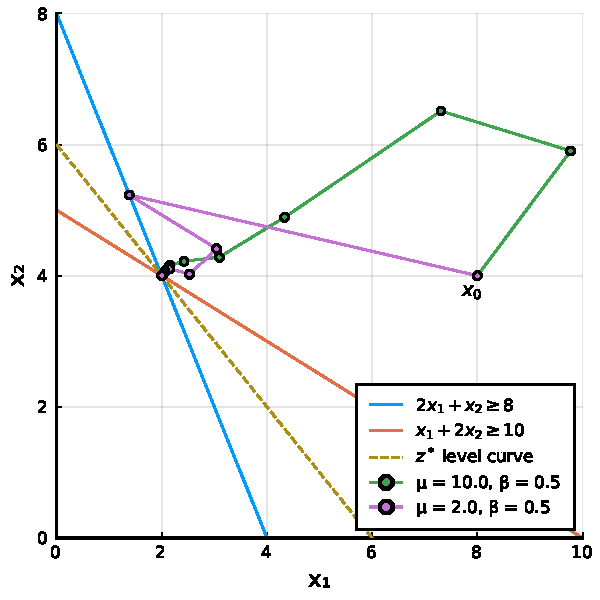
\includegraphics{part_2/chapter_10/figures/lp_example1-2.pdf}
\caption{IPM applied to a LP problem with two different barrier terms} \label{fig:lp_example1} 	
\end{figure}
%
Some points are worth noticing concerning Algorithm \ref{Alg2}. First, notice that in Line \ref{alg:w_update}, a fixed step size is considered. A line search can be incorporated to prevent infeasibility and improve numerical stability. Typically, it is used $\lambda^k_i = \min\braces{\alpha, - \frac{x_i^k}{d_i^k}}$ with $\alpha < 1$ but close to 1.

Also, even though the algorithm is initialised with a feasible solution $w^k$, this might in practice not be necessary. Implementations of the infeasible IPM method can efficiently handle primal and dual infeasibility.  

% Discuss surrogate dual in case of infeasible start IPM

Under specific conditions, the IPM can be shown to have complexity of $O(\sqrt{n}\ln(1/\epsilon))$, which is polynomial and of much better worst-case performance than the simplex method, which makes it the algorithm of choice for solving large-scale LPs. Another important advantage is that IPM can be modified with little effort to solve a wider class of problems under the class of \emph{conic optimisation problems}.

Predictor-corrector methods are variants of IPM that incorporate a two-phase direction calculation using a \emph{predicted} direction $d_w^{\text{pred}}$, calculated by setting $\mu=0$ and a \emph{correcting} direction, which is computed considering the impact that $d_w^{\text{cor}}$ would have in the term $\overline{X} \, \overline{U}e$.

Let $\Delta X = \diag(d_x^{\text{pred}})$ and $\Delta U = \diag(d_u^{\text{pred}})$. Then\\[-15pt]
\begin{align}
(X + \Delta X)(U + \Delta U)e &= XUe + (U \Delta X + X\Delta U)e + \Delta X \Delta U e\nonumber\\
& = XUe + (0 - XUe) + \Delta X \Delta U e\nonumber\\
& = \Delta X \Delta U e\label{eq:final}   
\end{align}
Using the last equation\hspace{-1.0pt}  \eqref{eq:final},\hspace{-1pt} the corrector Newton step becomes $\overline{U}d_x + \overline{X}d_u = \hat{\mu}e - \Delta X \Delta U e . 
$
Finally, $d_w^{k}$ is set to be a combination of $d_w^{\text{pred}}$ and $d_w^{\text{cor}}$. 
